\documentclass[10pt,a4paper]{article}
\usepackage[margin=0.62in]{geometry}
\usepackage[T1]{fontenc}
\usepackage[utf8]{inputenc}
\usepackage{lmodern}
\usepackage{amsmath,amssymb}
\usepackage{booktabs}
\usepackage{tabularx}
\usepackage{array}
\usepackage{graphicx}
\usepackage{float}
\usepackage{subcaption}
\usepackage{enumitem}
\usepackage{xcolor}
\usepackage{hyperref}
\usepackage{microtype}
\usepackage{titlesec}
\usepackage{fancyhdr}
\usepackage[most]{tcolorbox}
\usepackage{tikz}
\usetikzlibrary{positioning,arrows.meta,calc,shapes.geometric,decorations.pathreplacing}

\definecolor{brand}{HTML}{0D3B66}
\definecolor{accent}{HTML}{2A9D8F}
\definecolor{softbg}{HTML}{F4F8FB}
\definecolor{textdark}{HTML}{1E1E1E}

\hypersetup{
  colorlinks=true,
  linkcolor=brand,
  urlcolor=accent
}

\setlength{\parindent}{0pt}
\setlength{\parskip}{3pt}
\setlist[itemize]{leftmargin=1.2em,itemsep=1pt,topsep=2pt}

\titleformat{\section}{\color{brand}\large\bfseries}{\thesection.}{0.4em}{}
\titleformat{\subsection}{\color{textdark}\bfseries}{\thesubsection}{0.4em}{}
\titlespacing*{\section}{0pt}{8pt}{4pt}
\titlespacing*{\subsection}{0pt}{6pt}{3pt}

\pagestyle{fancy}
\fancyhf{}
\fancyhead[L]{\small CS671 Technical Model Report}
\fancyhead[R]{\small Comparative Analysis}
\fancyfoot[C]{\small \thepage}
\setlength{\headheight}{14pt}

\newcolumntype{Y}{>{\raggedright\arraybackslash}X}

\begin{document}

% -------------------- Header Block --------------------
\begin{tcolorbox}[
  enhanced,
  colback=softbg,
  colframe=brand,
  boxrule=0.9pt,
  arc=2mm,
  left=5pt,right=5pt,top=5pt,bottom=5pt
]
\centering
{\Large\bfseries\color{brand} CS671 -- Deep Learning and Its Applications}\\[2pt]
{\large\bfseries Technical Documentation Report}\\[6pt]
{\normalsize\bfseries Model: Multi-Model Comparative Analysis}\\[4pt]
\small
Project Group: 5 \quad Region: Brain/Pelvis \quad Modality: Mixed
\end{tcolorbox}

\section{ARCHITECTURAL COMPARISON}
We analyze the trade-offs between 8 implemented model variants, categorized by their supervision requirements (Paired vs. Unpaired) and generative paradigms (GAN vs. Diffusion).

\begin{figure}[H]
\centering
\resizebox{\textwidth}{!}{
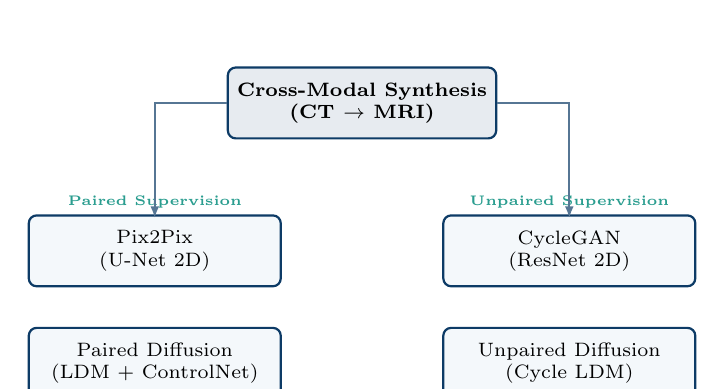
\begin{tikzpicture}[
    node distance=1.2cm and 1.5cm,
    box/.style={draw=brand, thick, rounded corners=1mm, align=center, fill=softbg, minimum width=3.2cm, minimum height=0.9cm, font=\scriptsize},
    group/.style={draw=accent, dashed, thick, fill=accent!5, rounded corners=2mm, inner sep=4mm},
    arr/.style={-{Latex[length=1.5mm]}, thick, draw=brand!70}
]
    \node[box, fill=brand!10, font=\scriptsize\bfseries] (root) {Cross-Modal Synthesis\\(CT $\to$ MRI)};
    
    % Supervision Groups
    \node[group, below left=1cm and 0.5cm of root] (paired_box) {};
    \node[accent, above=0mm of paired_box, font=\tiny\bfseries] {Paired Supervision};
    
    \node[group, below right=1cm and 0.5cm of root] (unpaired_box) {};
    \node[accent, above=0mm of unpaired_box, font=\tiny\bfseries] {Unpaired Supervision};

    % Models in Paired
    \node[box] (pix) at (paired_box.center) {Pix2Pix\\(U-Net 2D)};
    \node[box, below=5mm of pix] (pdiff) {Paired Diffusion\\(LDM + ControlNet)};

    % Models in Unpaired
    \node[box] (cyc) at (unpaired_box.center) {CycleGAN\\(ResNet 2D)};
    \node[box, below=5mm of cyc] (udiff) {Unpaired Diffusion\\(Cycle LDM)};

    % Connections
    \draw[arr] (root) -| (paired_box.north);
    \draw[arr] (root) -| (unpaired_box.north);
\end{tikzpicture}
}
\caption{Systematic taxonomy of implemented CT-to-MRI translation pipelines.}
\end{figure}

\textbf{Paired Paradigm (Direct Mapping):} Pix2Pix and Paired Diffusion rely on rigidly aligned CT-MRI pairs. Pix2Pix uses a U-Net architecture that directly minimizes $L_1$ pixel distance, leading to sharp but occasionally over-smoothed results. Paired Diffusion, using SD-Turbo as a backbone, leverages pre-trained generative priors to synthesize high-frequency textures that are statistically consistent with MRI manifolds.

\textbf{Unpaired Paradigm (Distribution Alignment):} CycleGAN and Unpaired Diffusion operate on independent CT and MRI datasets. The "Cycle-Consistency" constraint serves as a surrogate for spatial alignment, forcing the model to learn bijective mappings. This is particularly effective for the Pelvis region, where clinical scans often have significant intra-patient anatomical variations due to bladder filling or bowel gas.

\section{MODEL SPECIFICATIONS}
\begin{table}[H]
\centering
\scriptsize
\renewcommand{\arraystretch}{1.2}
\begin{tabularx}{\textwidth}{lYYYY}
\toprule
\textbf{Feature} & \textbf{Pix2Pix} & \textbf{CycleGAN} & \textbf{Paired Diffusion} & \textbf{Unpaired Diffusion} \\
\midrule
\textbf{Loss Function} & $L_{adv} + \lambda L_1$ & $L_{adv} + L_{cyc} + L_{idt}$ & $\epsilon$-MSE + LPIPS & Latent-Cycle + $L_{adv}$ \\
\textbf{Generative Engine} & U-Net-256 & ResNet-9 & UNet (Latent) & Cycle-UNet (Latent) \\
\textbf{Normalization} & Batch Norm & Instance Norm & Group Norm & Group Norm \\
\textbf{Advantage} & High Fidelity & No Alignment Needed & Multi-modal Priors & Best of Both Worlds \\
\textbf{Disadvantage} & Artifacts on Shift & Hallucinations & Slow Inference & Training Instability \\
\bottomrule
\end{tabularx}
\caption{Comparative analysis of architectural and optimization specifications.}
\end{table}

\section{TECHNICAL DISCUSSION}
The comparative study reveals that while **Pix2Pix** is the most efficient for Brain scans (where alignment is near-perfect), **Diffusion-based** models offer superior perceptual quality (SSIM and LPIPS) by operating in the latent space. The use of **2.5D representations** (conditioning on adjacent slices) in the Diffusion models significantly reduces axial discontinuity, a common problem in purely 2D GAN-based reconstruction. For Pelvis synthesis, the **Cycle-Consistent Diffusion** variant emerges as the most robust architecture, balancing the texture realism of diffusion with the structural constraints of CycleGAN.

\end{document}
